\section{Emuladores estoc\'asticos e aprendizado de m\'aquina}\label{sec:emuladores}

% Teoria do emulador (portada da Section_4 do grupo): simulador
% estocastico, GLD, metodo dos momentos e acoplamento com PCE. O
% procedimento CONCRETO de construcao (DoE, replicas, camada temporal)
% foi levado para a Metodologia (Secao~\ref{sec:metodologia}).

O elevado custo computacional de modelos de alta fidelidade frequentemente inviabiliza simulações diretas de Monte Carlo, exigindo o uso de metamodelos, também chamados de emuladores. Embora Processos Gaussianos (GP) \parencite{rasmussen2006} e Expansões em Caos Polinomial (PCE) \parencite{xiu2002} sejam padrão para sistemas determinísticos, eles não podem ser aplicados diretamente a simuladores estocásticos, nos quais uma única avaliação é insuficiente para caracterizar a distribuição da resposta.

\subsection{Simuladores estoc\'asticos}
\label{subsec:simulador}

Matematicamente, um simulador estocástico $\mathcal{M}_S$ pode ser visto como um mapeamento que incorpora variáveis determinísticas e aleatoriedade intrínseca. Para um dado vetor de parâmetros de entrada $\mathbf{x}$ no domínio $\mathcal{D}_X$, a resposta não é um valor determinístico único, mas uma variável aleatória $Y_{\mathbf{x}}$. Essa relação é formalmente expressa como:

\begin{equation}
\mathcal{M}_S : \mathcal{D}_X \times \Omega \rightarrow \mathbb{R}, \qquad (\mathbf{x}, \omega) \mapsto \mathcal{M}_S(\mathbf{x}, \omega),
\label{eq:simulador_estocastico}
\end{equation}

\noindent em que $\mathbf{x}$ representa o conjunto de parâmetros de entrada controlados (e.g., geometria, propriedades dos materiais) e $\omega$ denota um evento aleatório do espaço de probabilidade $\Omega$. Essa variável latente $\omega$ introduz a estocasticidade no sistema. Consequentemente, para uma entrada fixa $\mathbf{x}$, o simulador produz uma distribuição de resultados possíveis, e não uma solução única. No problema em estudo, $\mathcal{M}_S(\mathbf{x}, \omega) = g(\mathbf{x}, t; \omega)$ é a função de estado limite definida na Equação ~\eqref{eq:funcao_g}, e as variáveis latentes correspondem às incertezas de modelo e às flutuações não explicitamente parametrizadas.

\subsection{Distribuição Lambda Generalizada}
\label{subsec:gld}

No contexto da avaliação de durabilidade do concreto armado, o processo de carbonatação é influenciado por diversas fontes de incerteza, que vão da heterogeneidade do material às flutuações ambientais. Para capturar esses comportamentos probabilísticos complexos sem o custo computacional de simulações exaustivas, este estudo emprega a Distribuição Lambda Generalizada (GLD) como núcleo do emulador estocástico. A GLD é uma família de distribuições de quatro parâmetros, altamente flexível, projetada para aproximar uma ampla gama de distribuições paramétricas \parencite{KarianDudewicz2000, ZhuSudret2021}.

A GLD é definida por sua \textit{função quantílica} $Q(u)$, que é a inversa da função de distribuição acumulada (CDF), i.e., $Q(u) = F^{-1}(u)$. Essa abordagem é particularmente vantajosa para a emulação estocástica, pois facilita o método de amostragem por transformada inversa. Neste estudo, considera-se a família Freimer--Kollia--Mudholkar--Lin (FKML) \parencite{Freimer1988}, definida como:

\begin{equation}
Q(u) = \lambda_1 + \frac{1}{\lambda_2} \left( \frac{u^{\lambda_3} - 1}{\lambda_3} - \frac{(1 - u)^{\lambda_4} - 1}{\lambda_4} \right)
\label{eq:GLD_quantile}
\end{equation}

\noindent em que $u \in [0, 1]$ representa a probabilidade acumulada. A distribuição é governada por quatro parâmetros: $\lambda_1$ é o parâmetro de \textit{locação}, $\lambda_2$ é o parâmetro de \textit{escala} (com a exigência $\lambda_2 > 0$) e $\lambda_3, \lambda_4$ são os parâmetros de \textit{forma}.

\subsection{Estima\c{c}\~ao de par\^ametros via m\'etodo dos momentos}
\label{subsec:mom}

Para calibrar o emulador GLD, os quatro parâmetros $\boldsymbol{\lambda} = \{\lambda_1, \dots, \lambda_4\}$ devem ser estimados a partir de um conjunto de avaliações do modelo \parencite{karian2010handbook, corlu2016}. Neste estudo, emprega-se o \textit{Método dos Momentos} (MoM) \parencite{lakhany2000}, que consiste em igualar os momentos teóricos da GLD aos momentos empíricos calculados do conjunto amostral $\mathcal{Y} = \{y^{(1)}, \dots, y^{(N)}\}$. Os quatro primeiros momentos centrais --- média $\mu$, variância $\sigma^2$, assimetria $\delta$ e curtose $\kappa$ --- relacionam-se analiticamente aos parâmetros $\lambda$ da seguinte forma:

\begin{align}
\mu &= \lambda_1 - \frac{1}{\lambda_2} \left( \frac{1}{\lambda_3 + 1} - \frac{1}{\lambda_4 + 1} \right) \label{eq:mean} \\
\sigma^2 &= \frac{v_2 - v_1^2}{\lambda_2^2} \label{eq:variance_gld} \\
\delta &= \frac{v_3 - 3v_1v_2 + 2v_1^3}{(v_2 - v_1^2)^{3/2}} \label{eq:skew} \\
\kappa &= \frac{v_4 - 4v_1v_3 + 6v_1^2v_2 - 3v_1^4}{(v_2 - v_1^2)^2} \label{eq:kurt}
\end{align}

Nessas expressões, $v_k$ denota uma função não linear que depende apenas de $\lambda_3$ e $\lambda_4$, dada pela Equação~\eqref{eq:vk}, em que $B(\cdot, \cdot)$ representa a função Beta:

\begin{equation}
v_k = \sum_{j=0}^{k} \frac{(-1)^j}{\lambda_3^{k-j} \lambda_4^j} \binom{k}{j} B\!\left(\lambda_3(k-j) + 1,\; \lambda_4 j + 1\right) \label{eq:vk}
\end{equation}

A calibração dos parâmetros da GLD é formulada como um problema inverso, cujo objetivo é minimizar a discrepância entre os momentos analíticos (Equações~\ref{eq:mean}--\ref{eq:kurt}) e os momentos empíricos derivados do simulador estocástico. Para resolver esse sistema não linear, emprega-se o algoritmo de otimização Broyden--Fletcher--Goldfarb--Shanno (BFGS) \parencite{nocedal2006}, um método quase-Newton particularmente adequado a esse tipo de estimação devido ao tratamento eficiente de gradientes e às boas propriedades de convergência em espaços multidimensionais. O procedimento numérico foi implementado no PyGLAM, biblioteca Python desenvolvida pelos autores especificamente para a emulação de simuladores estocásticos com Distribuições Lambda Generalizadas.

Cabe registrar que o arcabouço GLaM original \parencite{ZhuSudret2021} emprega máxima verossimilhança condicional combinada a mínimos quadrados generalizados para a estimação dos parâmetros, dispensando réplicas no plano de experimentos. A opção pelo MoM com réplicas adotada neste trabalho justifica-se (i) pela robustez e simplicidade de implementação, (ii) pelo baixo custo de cada avaliação dos modelos mecânicos aqui considerados, que torna as réplicas viáveis, e (iii) pelo controle direto da qualidade do ajuste local em cada ponto do plano de experimentos, requisito importante para a camada temporal descrita na Seção~\ref{subsec:construcao_emulador}.

A acurácia desse ajuste --- que condiciona a de todo o arcabouço, por ser ele que converte cada conjunto de réplicas do simulador em um vetor $\boldsymbol{\lambda}$ --- é verificada de forma isolada na Seção~\ref{subsec:pyglam}, por meio do ajuste a distribuições de referência com solução analítica conhecida.

\subsection{Acoplamento com a Expans\~ao em Caos Polinomial}
\label{subsec:pce}

Seguindo a metodologia proposta por \textcite{ZhuSudret2021} e desenvolvimentos posteriores em metamodelagem estocástica, a GLD é acoplada à Expansão em Caos Polinomial (PCE) para a construção de um emulador global. Nesse arcabouço, a resposta estocástica do simulador para qualquer entrada $\mathbf{X}$ é modelada por uma GLD cujos parâmetros $\boldsymbol{\lambda}$ são, eles próprios, funções das variáveis de entrada.

Dado um conjunto de parâmetros de entrada $\mathbf{X}$ governado por uma função densidade de probabilidade conjunta $f_{\mathbf{X}}(\mathbf{x})$, cada componente do vetor de parâmetros $\lambda_i$ é aproximada por uma PCE truncada:

\begin{equation}
\lambda_i(\mathbf{X}) \approx \sum_{\boldsymbol{\alpha} \in \mathcal{A}} a_{i, \boldsymbol{\alpha}} \Psi_{\boldsymbol{\alpha}}(\mathbf{X}), \quad i = \{1, 2, 3, 4\}
\label{eq:pce_lambda}
\end{equation}

\noindent em que $\Psi_{\boldsymbol{\alpha}}(\mathbf{X})$ são polinômios ortonormais multivariados específicos das distribuições de entrada \parencite{xiu2002}, $a_{i, \boldsymbol{\alpha}}$ são os coeficientes a determinar e $\mathcal{A}$ é o conjunto de multi-índices que define o esquema de truncamento (e.g., base de grau total) \parencite{blatman2011}. Uma vez estimados os coeficientes, o emulador PCE--GLD fornece instantaneamente a distribuição de probabilidade completa (via parâmetros $\lambda$) para qualquer nova entrada $\mathbf{X}^*$, sem exigir novas execuções do simulador estocástico original. O procedimento concreto de construção do emulador --- plano de experimentos, réplicas estocásticas e extensão temporal --- é detalhado na Seção~\ref{subsec:construcao_emulador}.

\subsection{Aprendizado de m\'aquina como camada temporal}\label{sec:ml}

O emulador PCE--GLD descrito nas subseções anteriores fornece, para cada ponto do plano de experimentos e para cada instante simulado, um vetor de parâmetros $\boldsymbol{\lambda}$ que caracteriza a distribuição condicional da margem de segurança. Para que esse emulador opere de forma \textit{contínua} no tempo --- e não apenas nos instantes efetivamente simulados ---, é necessária uma camada de regressão capaz de aprender o mapeamento entre as variáveis de entrada, o tempo e os parâmetros da distribuição. Esta subseção apresenta os fundamentos de aprendizado de máquina empregados nessa camada, com ênfase nas redes neurais artificiais.

\subsubsection{Regress\~ao supervisionada de m\'ultiplas sa\'idas}
\label{subsec:ml_fundamentos}


\begin{equation}
\mathbf{w}^{*} = \argmin_{\mathbf{w}} \; \frac{1}{K}\sum_{k=1}^{K} \mathcal{L}\!\left(\boldsymbol{\lambda}^{(k)},\, \mathcal{M}_{ML}(\mathbf{z}^{(k)};\mathbf{w})\right) + \Omega(\mathbf{w}),
\label{eq:ml_treinamento}
\end{equation}

\noindent em que $\Omega(\mathbf{w})$ é um termo de regularização que penaliza a complexidade do modelo e mitiga o sobreajuste. Diferentemente da regressão determinística usual, aqui a variável-alvo não é a resposta física em si, mas os \textit{parâmetros de uma distribuição de probabilidade}; a acurácia da camada de ML traduz-se, portanto, diretamente na qualidade da distribuição emulada e, consequentemente, na estimativa de probabilidade de falha e de RUL.

Diversos regressores podem representar esse mapeamento, entre eles florestas aleatórias, regressão por vetores de suporte e redes neurais artificiais. Nos exemplos deste trabalho adota-se uma rede do tipo perceptron multicamadas para cada um dos dois parâmetros preditos, com arquitetura mantida entre o problema de referência e o de durabilidade. Essa definição constitui a configuração do experimento, sem uma comparação de desempenho entre famílias de regressores.

\subsubsection{Redes neurais artificiais}
\label{subsec:redes_neurais}


Inspiradas na biologia do cérebro humano, as redes neurais funcionam através de unidades básicas de processamento conhecidas como neurônios artificiais. Assim como os dendritos e sinapses biológicas recebem e modulam sinais elétricos, o modelo computacional recebe dados numéricos de entrada e aplica "pesos" matemáticos para determinar a importância relativa de cada variável. O verdadeiro poder dessa tecnologia reside em sua capacidade inata de generalização; após processar milhares de exemplos, a rede ajusta seus parâmetros e adquire a habilidade de prever respostas estruturais para cenários físicos inéditos com notável resiliência.

Para realizar esse mapeamento complexo, a arquitetura padrão organiza os neurônios em camadas hierárquicas, movimentando a informação unidirecionalmente da camada de entrada até a previsão final na camada de saída. A estrutura básica de uma rede neural é composta por um grande número de nós interconectados distribuídos nessas camadas, que se diferenciam fundamentalmente em três tipos: a camada de entrada (que capta as variáveis iniciais do projeto), as camadas ocultas (que realizam o processamento denso e a extração de padrões profundos) e a camada de saída (que emite a resposta final do modelo). O mecanismo de funcionamento da rede neural baseia-se na propagação contínua do sinal numérico através dessas conexões. O processamento matemático ocorre em duas etapas essenciais dentro de cada nó: primeiro, o neurônio realiza uma soma linear das entradas ponderadas pelos pesos, adicionando um valor de viés. Em seguida, o resultado passa por uma função de ativação não linear (como o ReLU), o que permite ao modelo emancipar-se das regressões simples e simular comportamentos não lineares de materiais, como a plasticidade do aço ou a fissuração do concreto. Adicionalmente, os tipos de camadas de saída dependem diretamente da aplicação estrutural desejada: em problemas de regressão a camada de saída opera geralmente com ativações lineares.

\begin{figure}[htpb!]
    \centering
    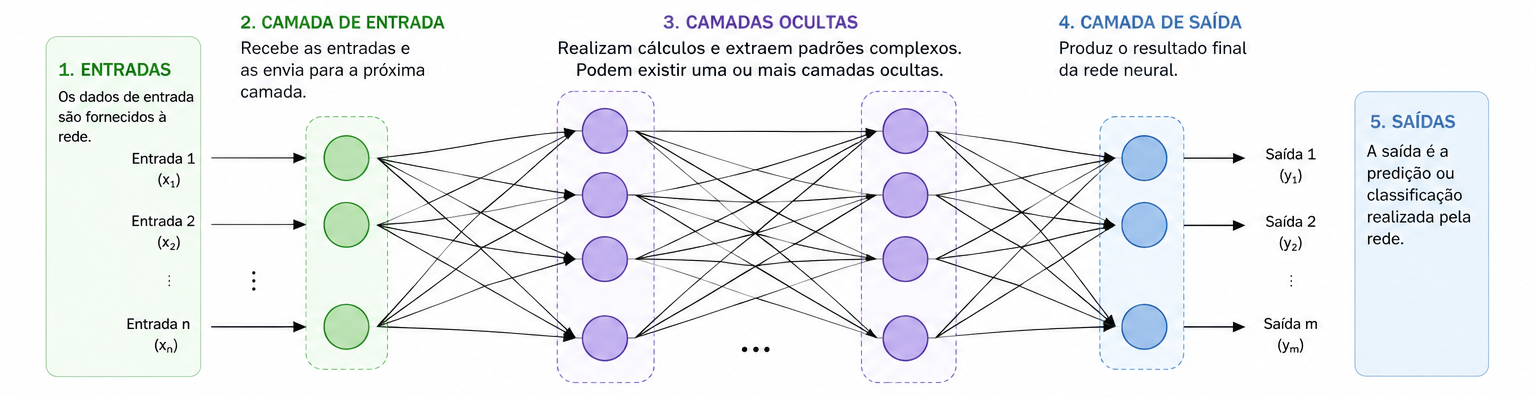
\includegraphics[width=1\linewidth]{z_fig_ANN.png}
    \caption{Diagrama de funcionamento de uma rede neural}
    \label{fig:diag_ANN}
\end{figure}


O "conhecimento" da rede neural é construído durante um processo chamado de treinamento supervisionado. No início, como os pesos internos são aleatórios, as previsões do modelo são bastante imprecisas, gerando a necessidade de medir a divergência em relação ao resultado real por meio de uma função de perda. O algoritmo então utiliza um método de retropropagação para avaliar as falhas e ajustar iterativamente os pesos de cada conexão. Com a exposição contínua aos dados de treino, o erro matemático diminui progressivamente e a rede converge para um estado de estabilidade, atingindo a precisão necessária para o uso na engenharia em tempo real.

As redes neurais artificiais são aproximadores universais de funções, capazes de representar mapeamentos não lineares arbitrariamente complexos desde que dotadas de capacidade suficiente. Uma rede do tipo perceptron de múltiplas camadas (\textit{Multilayer Perceptron} --- MLP) organiza-se em uma camada de entrada, uma ou mais camadas ocultas e uma camada de saída. Cada neurônio de uma camada $\ell$ computa uma combinação afim das ativações da camada anterior, seguida da aplicação de uma função de ativação não linear $\phi(\cdot)$:

\begin{equation}
\mathbf{a}^{(\ell)} = \phi\!\left(\mathbf{W}^{(\ell)} \mathbf{a}^{(\ell-1)} + \mathbf{b}^{(\ell)}\right), \qquad \mathbf{a}^{(0)} = \mathbf{z},
\label{eq:mlp_forward}
\end{equation}

\noindent em que $\mathbf{W}^{(\ell)}$ e $\mathbf{b}^{(\ell)}$ são, respectivamente, a matriz de pesos e o vetor de vieses da camada $\ell$, agrupados no conjunto de parâmetros $\mathbf{w} = \{\mathbf{W}^{(\ell)}, \mathbf{b}^{(\ell)}\}_\ell$. Funções de ativação usuais nas camadas ocultas incluem a unidade linear retificada (ReLU), $\phi(s) = \max(0,s)$, e a tangente hiperbólica, $\phi(s) = \tanh(s)$; a camada de saída, no caso de regressão, emprega tipicamente ativação linear. A saída da rede, $\mathbf{a}^{(L)}$, fornece a estimativa dos parâmetros $\hat{\boldsymbol{\lambda}}$.

O treinamento consiste na minimização da perda da Equação~\eqref{eq:ml_treinamento}, tipicamente o erro quadrático médio, por meio de \textit{retropropagação} do gradiente combinada a um otimizador de gradiente estocástico (e.g., Adam). Para evitar o sobreajuste, empregam-se estratégias de regularização como parada antecipada (\textit{early stopping}), penalização $\ell_2$ dos pesos e, quando pertinente, \textit{dropout}. A partição dos dados em subconjuntos de treinamento, validação e teste, aliada a validação cruzada, sustenta a estimativa honesta do erro de generalização.

Uma particularidade do presente problema é a condição $\lambda_2>0$ necessária à validade da GLD. Na implementação utilizada, os alvos são previstos diretamente, sem transformação logarítmica nem ativação positiva na saída. A base temporal de durabilidade exclui alvos com $\lambda_2\leq0$, mas isso não garante a positividade de novas predições. Nos diagnósticos distribucionais, predições inválidas são identificadas e retornam métricas ausentes; sua ocorrência e localização devem ser reportadas. Os parâmetros de forma são mantidos nos valores fixos informados em cada exemplo.

No arcabouço proposto, cada RNA recebe o vetor $\mathbf{z}=(\mathbf{x},t)$ e prediz um dos parâmetros $\lambda_1$ ou $\lambda_2$. São utilizadas duas camadas ocultas de 64 neurônios, implementadas com \texttt{MLPRegressor} da biblioteca \texttt{scikit-learn}, padronização das entradas e parada antecipada. O procedimento de construção dos alvos e a partição dos dados são detalhados nas Seções~\ref{subsub:temporal} e~\ref{subsec:exemplo2}.
